
\section{Efectuarea lucrarii de laborator}



\subsection{Tasks and Points}



Basic Level (nota 5 $||$ 6) : 

-initializeaza un nou repositoriu

-configureaza-ti VCS

-crearea branch-urilor (creeaza cel putin 2 branches)

-commit pe ambele branch-uri (cel putin 1 commit per branch)



Normal Level (nota 7 $||$ 8):
 
-seteaza un branch to track a remote origin pe care vei putea sa faci push (ex. Github, Bitbucket or custom server)

-reseteaza un branch la commit-ul anterior

-salvarea temporara a schimbarilor care nu se vor face commit imediat.

-folosirea fisierului .gitignore



Advanced Level (nota 9 $||$ 10):

-merge 2 branches

-rezolvarea conflictelor a 2 branches

-comezile git care trebuie cunoscute 

Bonus Point (+1):

-Tags. Folosirea tag-urilor pentru marcarea schimbarilor simnificative precum release-ul.



\subsection{Analiza lucrarii de laborator}


Linkul la repozitoriu: \texttt{https://github.com/dumitritag/MIDPS-lab}

1.Initializarea unui repositoriu si configurarea VCS

 Initial a fost creat un cont pe GitHub care contine repozitoriul laboratorului efectuat. Am creat repozitoriul meu \textit {MIDPS$-$lab}. A fost stabilita conexiunea cu serverul prin generarea keygen-ului SSH prin instructiunea \textit {ssh-keygen}, ea fiind adaugata in setari.  Dupa ce am clonat repozitoriul, folosind comanda \textit {git clone shhlik} , am configurat contul cu comenzile \textit {git config $-$global user.name "YourName"} si \textit {git config $-$global user.email "youremail@domain.com"}  Am creat fisierele .gitignore si README in repozitoriu si cu ajutorul comenzii \textit {git pull} le-am adaugat in masina locala. In masina locala am creat 5 mape, fiecare continind cite un fiser README si le-am adaugat in repozitoriu cu comenzile \textit {git add .} , \textit {git commit} si \textit {git push} . Commiturile sunt schimbarile salvate in poiectu nostru. Fiecare commit are un mesaj asociat, in care descrim ce schimbare am facut. In mapa Lab1 din masina locala am creat un fisier myfile.txt cu continutul "Welcome!" si l-am adaugat in repozitoriu.

2. Crearea branch-urilor 

Branch-ul implicit in Git este master, comanda \textit {git init} il creeaza implicit. Am creat 2 branch-uri noi: branch1 si branch2 cu ajutorul comenzii \textit {git branch <branchname>}. Aceasta creeaza un nou pointer la ultimul commit. Pentru a comuta la un branch nou am folosit comanda \textit {git checkout <branchname>}. Am modificat fisierul myfile.tx, l-am adaugat la branch-urile si am facut primele commituri in noile branch-uri.

3. Track remote origin

 Am creat un nou branch newbranch  to track remote origin, folosind comanda \textit {git branch --track <branchname> origin/master}. Am creat un nou fisier new.txt, l-am adaugat, am facut commit si cu comanda \textit {git push origin <branchname>} am adaugat commitul in newbranch iar cu comanda \textit {git push origin HEAD:master} in master branch.
 
 4. Resetarea unui branch la commitul anterior
 
 Pentru rescrierea commitului anterior am folosit comanda \textit {git commit --amend}. Pentru resetarea unui branch la commitul anterior am folosit comanda \textit {git revert HEAD}.
 
 5. Salvarea temporara a schimbarilor
 
 Uneori facem schimbari care nu dorim sa le facem commit dar dorim sa le salvam, asta putem face cu comanda \textit {git stash}.
 
 6. Folosirea fisierului .gitignore
 
 Pentru a vedea cum influenteaza fisierul .gitignore, am adaugat in fisierul .gitignore *.txt si am creat un nou fisier de tip txt, am aplicat comanda git add si acest fisier a fost ignorat.
 
 7. Merge 2 branches
 
 Merge 2 branches inseamna a le integra intr-un singur branch. Pentru aceasta am folosit comanda \textit {git merge <branchname>}.
 
 8. Rezolvarea conflictelor a 2 branch-uri
 
 Daca avem 2 branches, in ambele a fost schimbat aceeasi parte a unui fisier si dorim sa facem merge la ambele va aparea un conflict. Acest conflict putem sa-l rezolvam manual, modificind fisierul care a cauzat conflictul. O alta metoda este prin folosirea comenzii \textit {git rebase master}. 
 
 9. Folosirea tag-urilor
 
 Un tag este folosit pentru a eticheta si a marca un commit. Sunt 2 tipuri de tag-uri lightweight, folosim comanda \textit {git tag <tagname>} si annotated, comanda folosita este \textit {git tag -am "message" <tagname>}.
 
 
\clearpage


\subsection{Imagini}



1. Crearea branch-lor noi

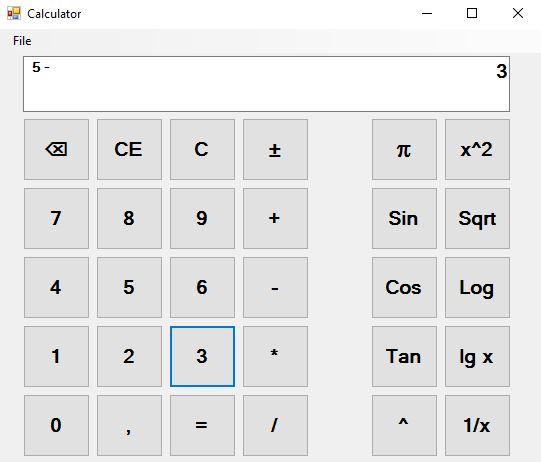
\includegraphics{Cattura1.JPG}

2. Commit in branch1

\includegraphics{Cattura1a.JPG}

\clearpage

3. Commit in branch 2

\includegraphics{Cattura1b.JPG}

4. Track remote origin

\includegraphics{Cattura1c.JPG}

\includegraphics{Cattura1d.JPG}

\includegraphics{Cattura1e.JPG}

5. Redenumirea unui commit

\includegraphics{Cattura1h.JPG}

\includegraphics{Cattura1f.JPG}

\clearpage

6. Resetarea la commitul anterior

\includegraphics{1.JPG}

\includegraphics{2.JPG}

\includegraphics{3.JPG}

7. Salvarea temporara a schimbarilor

\includegraphics{Cattura1m.JPG}

\includegraphics{Cattura1n.JPG}

8. Folosirea fisierului .gitignore

\includegraphics{Cattura1r.JPG}

9. Merge 2 branches

\includegraphics{Cattura1t.JPG}

\clearpage

10. Rezolvarea conflictelor 

Manual:

\includegraphics{Cattura1q.JPG}

\includegraphics{Cattura1y.JPG}

\includegraphics{Cattura1x.JPG}

Comanda git rebase:

\includegraphics{Cattura1yy.JPG}

\includegraphics{Cattura1yyyyyy.JPG}

\includegraphics{Cattura1yyyy.JPG}

11. Tags

\includegraphics{Cattura1xx.JPG}

\includegraphics{Cattura1wwww.JPG}

\includegraphics{Cattura1yyyyyyyy.JPG}

\includegraphics{Cattura1www.JPG}



\clearpage
        
